\documentclass[crop,tikz]{standalone}
\usetikzlibrary{backgrounds}
\colorlet{blue}{cyan}
\tikzset{
  inverted/.style = {
    every path/.style = {draw=white,text=white},
    background rectangle/.style={fill},
    show background rectangle
  }
}

\tikzset{>=latex}
\colorlet{blue}{blue!70!green}

\begin{document}
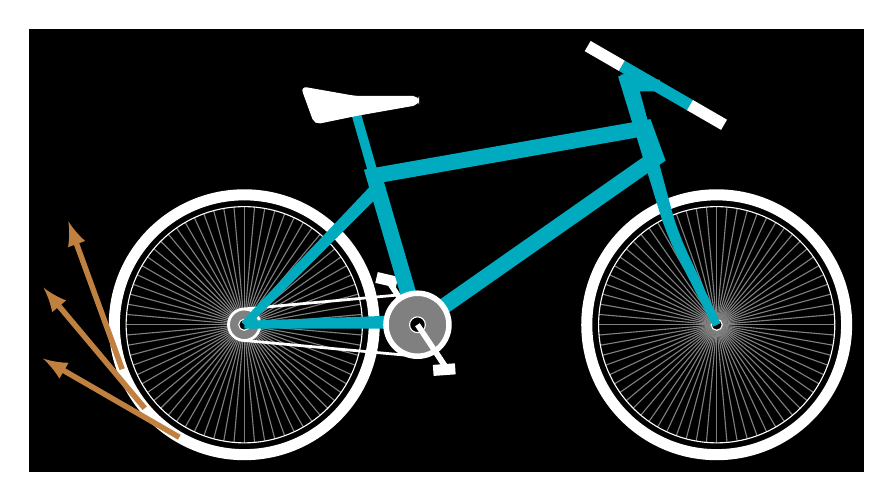
\begin{tikzpicture}[inverted,inverted]
  \def\WheelRadiusInner{1.5cm}
  \def\WheelRadiusOuter{\WheelRadiusInner+0.15cm}
  \def\PetalRadius{0.4cm}
  % wheel 1
  \coordinate (wheel1) at (0,0);
  \foreach \a in {0,5,...,355} {
    \draw[gray] (wheel1) -- (\a:\WheelRadiusInner);
  }
  \draw[line width=4pt] (wheel1) circle (\WheelRadiusOuter); % outer
  \draw (wheel1) circle (\WheelRadiusInner); % inner
  \draw[fill=gray,line width=1pt] (wheel1) circle (0.2cm); % inner
  \fill (wheel1) circle (2pt); % inner
  % wheel 2
  \coordinate (wheel2) at (6,0);
  \foreach \a in {0,5,...,355} {  
    \draw[gray] (wheel2) -- ++(\a:\WheelRadiusInner);
  }
  \draw[line width=4pt] (wheel2) circle (\WheelRadiusOuter); % outer
  \draw (wheel2) circle (\WheelRadiusInner); % inner
  \fill (wheel2) circle (2pt); % inner
  % chain
  \coordinate (petal) at (2.2,0);
  \draw[line width=1pt] (0,0.2cm)--(2.2,\PetalRadius) (0,-0.2cm)--(2.2,-\PetalRadius);
  % petal 1
  \draw[line width=2pt] (petal)--(2.6,-0.6) (petal)--(1.8,0.6);
  \draw[line width=4pt] (1.68,0.6)--(1.94,0.54);
  % handlebars
  \draw[blue,line width=1mm,rounded corners=8pt,rotate around={25:(wheel2)}] (wheel2)--(6,1.3cm)--++(80:2.1cm);
  \draw[blue,line width=1mm,rounded corners=8pt,rotate around={27:(wheel2)}] (wheel2)--(6,1.3cm)--++(80:2.1cm);
  \draw[blue,line width=1mm,rounded corners=8pt,rotate around={26:(wheel2)}] (wheel2)--(6,1.3cm)--++(80:2.1cm) coordinate (a);
  \draw[blue,line width=1.5mm] (a)--++(-80:0.15cm)--++(0:\PetalRadius)--++(180:0.05cm) coordinate (b);
  \draw[blue,line width=1.5mm] (b) -- ++(-30:0.5cm) coordinate (a);
  \draw[line width=1.5mm] (a) -- ++(-30:0.5cm);
  \draw[blue,line width=1.5mm] (b) -- ++(150:0.5cm) coordinate (a);
  \draw[line width=1.5mm] (a) -- ++(150:0.5cm);
  % chassis
  \draw[blue,line width=2mm,rotate around={35:(petal)}] (petal)--++(3.7,0)--++(75:0.4cm)--++(155:3.5)coordinate(e)--(petal);
  \draw[blue,line width=1mm] (0,0)--(petal) (0,0)--(45:2.5cm) (0,0)--(46.5:2.5) (0,0)--(2:2.2);
  \draw[blue,line width=1.2mm] (e)--++(106:0.9cm)--++(-74:0.1cm)coordinate(d);
  % chain--petal connection
  \draw[fill=gray,line width=2pt] (petal) circle (\PetalRadius);
  % petal 2
  \fill (petal) circle (0.1cm);
  \draw[line width=4pt] (2.4,-0.58)--(2.68,-0.56);
  \draw[line width=2pt] (petal)--(2.6,-0.6);
  % saddle
  \fill[white,rounded corners=2pt] (d)--++(10:0.8cm)--++(90:1mm)--++(180:0.8cm)--++(170:0.7cm)--++(-70:0.5cm)--cycle;
  % dirt
  \foreach \a in {240,220,200} {
    \draw[->,brown,line width=2pt] (wheel1)++(\a:\WheelRadiusOuter) -- ++(\a-90:2cm);
  }
\end{tikzpicture}
\end{document}
